s\begin{tikzpicture}[
  font=\sffamily,
  >=Latex,
  stage/.style={draw, rounded corners=2pt, thick, minimum width=36mm, minimum height=18mm, align=center},
  wire/.style={->, thick},
  smalltxt/.style={font=\scriptsize\sffamily},
  scale=0.5
]

% ---------- icon sizes ----------
\def\iconW{8mm}
\def\iconH{6.5mm}

% ---------- icons (no x1/x2 needed) ----------
\newcommand{\SineIcon}{%
  \begin{tikzpicture}[x=\iconW,y=\iconH,baseline=-0.5ex]
    \clip (0,0) rectangle (1,1);
    \draw[gray!50, line width=0.4pt] (0,0.5) -- (1,0.5);
    \draw[line width=0.8pt]
      plot[smooth, samples=60, domain=0:360]
      ({\x/360}, {0.5 + 0.35*sin(\x)});
  \end{tikzpicture}%
}

\newcommand{\FadeIcon}{%
  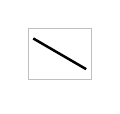
\begin{tikzpicture}[x=\iconW,y=\iconH,baseline=-0.5ex]
    \draw[gray!50, line width=0.4pt] (0,0) rectangle (1,1);
    \draw[line width=0.9pt] (0.08,0.80) -- (0.92,0.20);
  \end{tikzpicture}%
}

\newcommand{\ADSRIcon}{%
  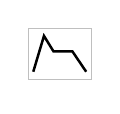
\begin{tikzpicture}[x=\iconW,y=\iconH,baseline=-0.5ex]
    \draw[gray!50, line width=0.4pt] (0,0) rectangle (1,1);
    \draw[line width=0.9pt]
      (0.08,0.15) --  % start
      (0.25,0.85) --  % attack
      (0.40,0.55) --  % decay
      (0.70,0.55) --  % sustain
      (0.92,0.15);    % release
  \end{tikzpicture}%
}

\def\sinicon#1#2{
    \textbf{#1}\\[-1pt]
    {\footnotesize #2}\\[-1pt]
    \SineIcon
}

\def\fadeicon#1#2{
  \textbf{#1}\\[-1pt]
  {\footnotesize #2}\\[-1pt]
  \FadeIcon
}

% ---------- nodes ----------

\node[stage] (tone) { \sinicon{t1}{\texttt{note * 0.997}} };
\node[stage, right=6mm of tone] (tone1) {\sinicon{t2}{\texttt{note * 1.001}}};
\node[stage, below=8mm of $(tone.south)!0.5!(tone1.south)$] (mix1) {\texttt{+}};
\node[stage, below=8mm of mix1] (fade) {\fadeicon{fade\_out}{\texttt{t}}};

\node[stage, right=6mm of tone1] (harmonic1) {\sinicon{harmonic1}{\texttt{note * 2.01}}};
\node[stage, below=4mm of harmonic1] (fade1) {\fadeicon{fade\_out}{\texttt{1.5 * t}}};

\node[stage, right=6mm of harmonic1] (harmonic2) {\sinicon{harmonic2}{\texttt{note * 3.05}}};
\node[stage, below=4mm of harmonic2] (fade2) {\fadeicon{fade\_out}{\texttt{2 * t}}};

\node[stage, right=6mm of harmonic2] (harmonic3) {\sinicon{harmonic2}{\texttt{note * 4.001}}};
\node[stage, below=4mm of harmonic3] (fade3) {\fadeicon{fade\_out}{\texttt{10 * t}}};

\node[stage, below=12mm of $(fade.south)!0.5!(fade3.south)$, xshift=5mm] (mix2) {\texttt{+}};
%\node[stage, right=16mm of mix] (adsr) {%
%  \textbf{adsr}\\[-1pt]
%  {\footnotesize $A,D,S,R$}\\[-1pt]
%  \ADSRIcon
%};
%
%\node[stage, right=16mm of adsr] (fade) {%
%  \textbf{fade\_out}\\[-1pt]
%  {\footnotesize $T=1.5\ \mathrm{s}$}\\[-1pt]
%  \FadeIcon
%};

%\node[stage, right=16mm of fade, minimum width=28mm] (play) {%
%  \textbf{play}\\[-1pt]
%  {\footnotesize speaker}
%};

% ---------- wires ----------
\draw[wire] (tone.south) to[out=-90,in=90,looseness=0.6] (mix1.north);
\draw[wire] (tone1.south) to[out=-90,in=90,looseness=0.6] (mix1.north);

\draw[wire] (mix1.south) to[out=-90,in=90,looseness=0.6] (fade.north);
\draw[wire] (harmonic1.south) to[out=-90,in=90,looseness=0.6] (fade1.north);
\draw[wire] (harmonic2.south) to[out=-90,in=90,looseness=0.6] (fade2.north);
\draw[wire] (harmonic3.south) to[out=-90,in=90,looseness=0.6] (fade3.north);

\draw[wire] (fade.south) to[out=-90,in=90,looseness=0.6] (mix2.north);
\draw[wire] (fade1.south) to[out=-90,in=90,looseness=0.6] (mix2.north);
\draw[wire] (fade2.south) to[out=-90,in=90,looseness=0.6] (mix2.north);
\draw[wire] (fade3.south) to[out=-90,in=90,looseness=0.6] (mix2.north);
%\draw[wire] (mix.east) -- (adsr.west);
%\draw[wire] (adsr.east) -- (fade.west);
%\draw[wire] (fade.east) -- (play.west);

% ---------- grouping box ----------
% \node[draw, thick, rounded corners=3pt, inner sep=5mm, fit=(tone)(tone2)(mix)(adsr)(fade), label={[font=\small\sffamily]above left:Instrument}] {};

\end{tikzpicture}
